This chapter provides an overview of the \ac{DT} concept,
its historical development and the more recent models and technologies that have emerged
to support its implementation.
%
The ever-growing literature on the subject reflects the increasing interest in \acp{DT}
and its multi-faceted nature, encompassing various domains and applications.
%
In this thesis we focus on the software engineering perspective of \acp{DT}, 
and the application of \acp{DT} to the engineering of \ac{IoT} systems.
%
Accordingly, this chapter focuses on how the \ac{DT} concept has been interpreted in this context.


%=======================================================
\section{History and Definitions}
%=======================================================

The concept of \ac{DT} was introduced in the early 2000s by Michael Grieves
in the context of Product-Lifecycle Management~\cite{Grieves_2023}
where it was conceived as a virtual representation of a product throughout its lifecycle.
%
At its essence, Grieves defined what later came to be known as a \ac{DT} as a system composed of three main components (\Cref{fig:dt-grieves-original}):
\begin{itemize}
\item a \emph{physical space} and its products;
\item a \emph{virtual space} containing the digital representation of the products;
\item a \emph{connection} between the two, making data flow from the physical to the virtual space and information flow from the virtual to the physical space~\cite{Grieves2017}.
\end{itemize}

\begin{figure}[ht]
    \centering
    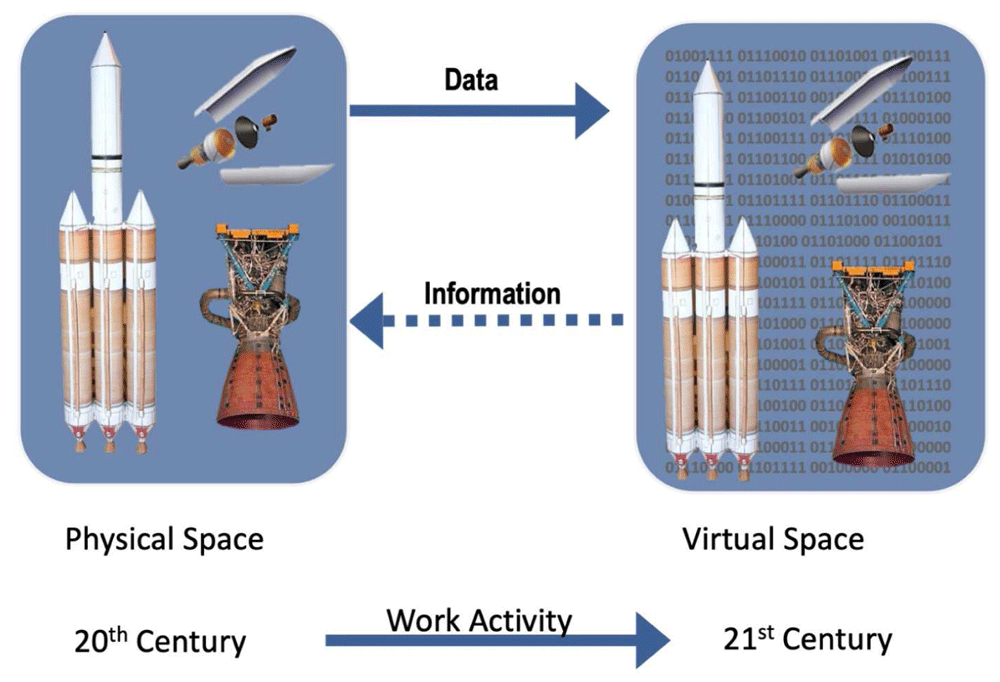
\includegraphics[width=0.7\textwidth]{figures/dt-original.png}
    \caption{The original \ac{DT} model by Grieves, from \cite{Grieves_2022}.}
    \label{fig:dt-grieves-original}
\end{figure}

Grieves referred to this concept as the \emph{Mirrored Spaces Model}~\cite{Grieves_2005},
a name which echoes the idea of \emph{Mirror Worlds} introduced by David Gelernter in the 1990s~\cite{gelernter1991mirrorworlds}
who also envisioned the ability to replicate the real world in a completely virtual space~\cite{Singh_Fuenmayor_Hinchy_Qiao_Murray_Devine_2021}.

The idea was later associated with its modern \emph{\acl{DT}} name and popularized by NASA in the 2010s, when it was presented as a key technology
for future development of aircraft and spacecraft in order to virtually simulate extreme conditions,
integrate data from the physical system in operation, 
and provide feedback on the conditions of the \emph{flying twin}
while possibly enacting changes to mitigate damage~\cite{glaessgen2012dtnasa}.
%
NASA's definition hence focused on the ability of the \ac{DT} to integrate multiple simulation models and characterized the \ac{DT} as \emph{ultra-realistic}, as the goal was to virtually replicate the physical system with the highest possible degree of fidelity:

\begin{quote}
    A Digital Twin is an integrated multiphysics, multiscale, probabilistic simulation of an as-built vehicle or system that uses the best available physical models, sensor updates, fleet history, etc., to mirror the life of its corresponding flying twin~\cite{glaessgen2012dtnasa}.
\end{quote}

Given the various phases of a product's lifecycle, the \ac{DT} concept was later
refined to distinguish between the \emph{Digital Twin Prototype} (DTP) and the \emph{Digital Twin Instance} (DTI) and \emph{Digital Twin Aggregate} (DTA)~\cite{Grieves2017}.
The DTP is the virtual representation of the product during its design and development phase,
while the DTI is the virtual representation of the product during its operational phase.
%
The DTA represents instead the aggregation of all DTIs, hence all products that have been built~\cite{Grieves_2022}.
%
Interestingly, the DTP exists before the physical product is even produced, 
and it is rather ``just'' a virtual model of the product. 
%
Grieves argues that requiring that a \ac{DT} exists only when the physical product exists is a \emph{fallacy}~\cite{Grieves_2022}.
%
Nevertheless, it is generally accepted within the community nowadays that, for a proper characterization, what is usually referred as \ac{DT} is hence a DTI, which exists alongside its physical counterpart and is continuously updated with data from the physical world. 

The role of such bidirectional data exchange between the physical and virtual parts
of a \ac{DT} has been, in fact, used to characterize the \ac{DT} concept and distinguish it from other related concepts.
%
A widely accepted taxonomy classifies the concepts of \emph{Digital Model}, \emph{Digital Shadow} and \emph{Digital Twin} based on direction of the automatic data flow between the physical and virtual spaces~\cite{kritzinger2018dtmanufacturing} (\Cref{fig:dt-taxonomy}):
namely, 
a Digital Model (\Cref{fig:dt-taxonomy-digital-model}) is a static model of a physical system (similarly to the DTP) that can be manually updated over time,
the Digital Shadow (\Cref{fig:dt-taxonomy-digital-shadow}) gets automatically updated through an inbound data flow from the physical space,
while the Digital Twin (\Cref{fig:dt-taxonomy-digital-twin}) is the only one that holds a bidirectional data flow which can provide feedback to the physical counterpart.
%
Such connection has been referred to as the \emph{digital thread}~\cite{Singh_Willcox_2018,Grieves_2023} to evoke the idea of a tie that binds the physical and virtual spaces.
%
Other common terms include \emph{twinning}~\cite{JONES202036} or \emph{shadowing}~\cite{Jiang_Yin_Li_Luo_Kaynak_2021,web-of-dt-ricci-2022} process. 
%
This terminology emphasizes the continuous and dynamic nature of the relationship between the physical and virtual entities, 
and highlights the active role of such process in maintaining the \ac{DT} up to date.

\begin{figure}[ht]
    \centering
    \begin{subfigure}[b]{0.3\linewidth}
        \centering
        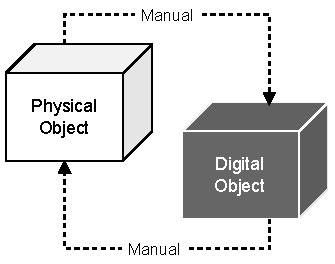
\includegraphics[width=\linewidth]{figures/kritzinger-digital-model.pdf}
        \caption{Digital Model}
        \label{fig:dt-taxonomy-digital-model}
    \end{subfigure}
    \hfill
    \begin{subfigure}[b]{0.3\linewidth}
        \centering
        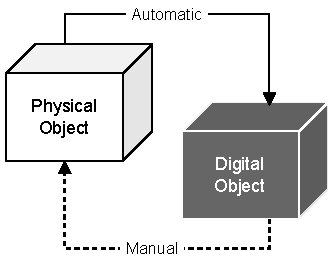
\includegraphics[width=\linewidth]{figures/kritzinger-digital-shadow.pdf}
        \caption{Digital Shadow}
        \label{fig:dt-taxonomy-digital-shadow}
    \end{subfigure}
    \hfill
    \begin{subfigure}[b]{0.3\linewidth}
        \centering
        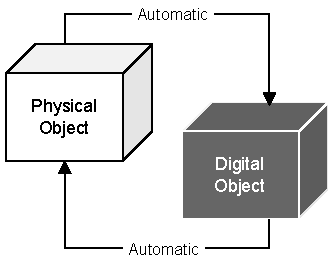
\includegraphics[width=\linewidth]{figures/kritzinger-digital-twin.pdf}
        \caption{Digital Twin}
        \label{fig:dt-taxonomy-digital-twin}
    \end{subfigure}
    \caption{Taxonomy of Digital Twin related concepts based on the data flows between physical and digital objects, adapted from \cite{kritzinger2018dtmanufacturing}.}
    \label{fig:dt-taxonomy}v
\end{figure}

The scope and applicability of the \ac{DT} concept has evolved and expanded
to encompass a wide range of applications and domains.
%
Today, \acp{DT} are used in various fields such as manufacturing, healthcare, smart cities, and more.
%
This is also reflected in the abundance of terminology used to identify the physical counterpart of a \ac{DT}
which is nowadays often referred to as the \emph{physical twin} or
\emph{physical entity}~\cite{Singh_Fuenmayor_Hinchy_Qiao_Murray_Devine_2021,JONES202036,DBLP:journals/jss/DaliborJRSWWW22}.
%
This shift from identifying the physical counterpart as a \emph{product} to a more generic \emph{entity}
highlights the broader applicability of the \ac{DT} concept beyond its original manufacturing context.
%
The \ac{DT} concept has been adopted also to represent people~\cite{Shengli_2021},
processes (e.g., supply chain~\cite{Barykin_Bochkarev_Kalinina_Yadykin_2020}) and organizations~\cite{Parmar_Leiponen_Thomas_2020}, leading to a more abstract interpretation of what can be considered \emph{physical}. 
%
Accordingly, the definitions of \acp{DT} have also diversified, leading to a plethora of interpretations~\cite{DBLP:journals/jss/DaliborJRSWWW22}. 

For the scope of this thesis, 
since the focus is on how \acp{DT} can be used to engineer \ac{IoT} systems, taking as the reference context the healthcare domain,
we adopt the following definition, adapted from \cite{dt-IoT-context-Minerva-2020}:

\begin{quote}
A \acf{DT} is a comprehensive software representation of an individual \acl{PA}.
It includes the properties, conditions, and behavior(s) of the real-life asset through models and data.
A \ac{DT} is a set of realistic models that can simulate an asset's behavior in the deployed environment.
The \ac{DT} represents and reflects its physical twin and remains its virtual counterpart across the asset's entire lifecycle.
\end{quote}

The definition emphasizes the software nature of the \ac{DT} and its ability to model the properties and behavior of its physical counterpart.
%
We deliberately use the term \emph{\ac{PA}} to refer to the physical counterpart of a \ac{DT}
to highlight the fact that an \emph{asset} is something that has a strategic
value in the context of an application domain, and that the \ac{DT} is meant to represent and manage such assets.
%
Compared to the original Grieves model which characterized the \ac{DT} as having three parts (physical, digital and connection), for the reminder of this thesis we will instead consider:
\begin{itemize}
\item the \ac{PA} as the physical counterpart of a \ac{DT};
\item the \ac{DT} as the software implementing the virtual representation of the \ac{PA} through a combination of models and data;
\item the \emph{twinning process} implemented by the \ac{DT} software to keep the \ac{DT} up to date with the \ac{PA} and possibly provide feedback to it.
\end{itemize}

%=======================================================
\section{Reference Architectures and Properties}
%=======================================================

The conceptual definition of \ac{DT} gives little indication on how to implement it,
leaving a degree of freedom in the technical realization of the \ac{DT} software.
%
For this reason, a variety of reference architectures have been proposed, 
each emphasizing different aspects of the \ac{DT} concept~\cite{ferko2022architecting}.

One that has gained significant recognition in the \ac{DT} community is the \emph{five-dimensional model} (5D model) by Tao et al.~\cite{dt-driven-prognostics-tao-2018}.
%
As shown in \Cref{fig:dt-5d-model}, the 5D model characterizes a \ac{DT} as composed of five main components~\cite{qi2021enablingtechdt}:
\begin{itemize}
\item the \emph{physical entity} (PE), which is the physical counterpart of the \ac{DT};
\item the \emph{virtual models} (VM), which is the digital representation of the PE possibly including 3D models, rules and behavioral models;
\item the \emph{data} (DD), which includes all data related to the PE and possibly generated by the VM, such as historical data, real-time data, simulation results;
\item the \emph{service} (Ss), which encompasses all services provided by the \ac{DT} to users, such as monitoring, simulation, diagnostics, and optimization;
\item the \emph{connection} (CN), which represents the communication and data exchange between all other components, there including the bidirectional connection between the PE and the VM that is fundamental for the \ac{DT} operation.
\end{itemize}

\begin{figure}[ht]
    \centering
    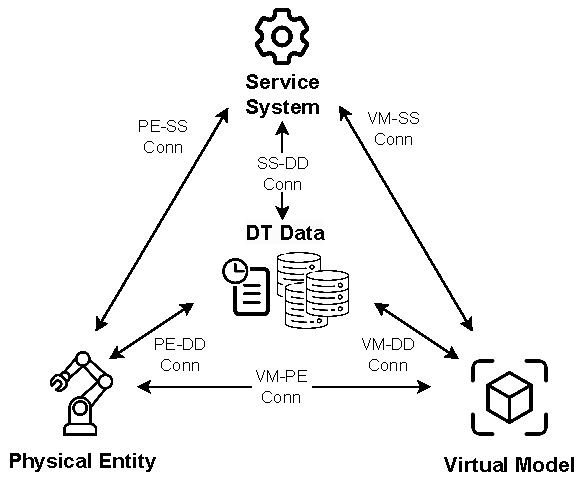
\includegraphics[width=0.6\textwidth]{figures/5d-model.pdf}
    \caption{The 5D model of a Digital Twin.}
    \label{fig:dt-5d-model}
\end{figure}

Tao's 5D model extends Grieves' original model by explicitly including the data and services dimensions, better characterizing the \ac{DT} as a data-driven and service-oriented system. 


The service-oriented nature of \acp{DT} has an essential role in their ability to provide value to users.
%
The \ac{DT} is hence not just a passive representation of a \ac{PA}, but an active system that users can interact with to obtain insights and perform actions on the \ac{PA}.
%
This also contrasts the idea of the \ac{PA}-\ac{DT} system as a closed-loop control system, but rather envisions the \ac{DT} as open to interactions with external entities such as human users or other software systems.

Following this perspective, the idea of \ac{DT}-as-a-service has been proposed.
As shown in \Cref{fig:dt-as-a-service}, the proposed reference architecture adds a cyber layer and an application layer on top of the classic physical, digital and communication layers of a \ac{DT}~\cite{aheleroff2021aei}.
%
The reference architecture further highlights different levels of integration following the taxonomy of Digital Model, Shadow, and Twin~\cite{kritzinger2018dtmanufacturing}, with a further Digital Twin predictive level, which includes predictive models and analytics capabilities enabled by the cyber layer grounded on cloud technologies such as Big Data analytics. 
%
The vision additionally integrates \acp{DT} in an incremental and iterative development lifecycle, to accompany and evolve alongside the \acp{PA} they represent. 

\begin{figure}[ht]
    \centering
    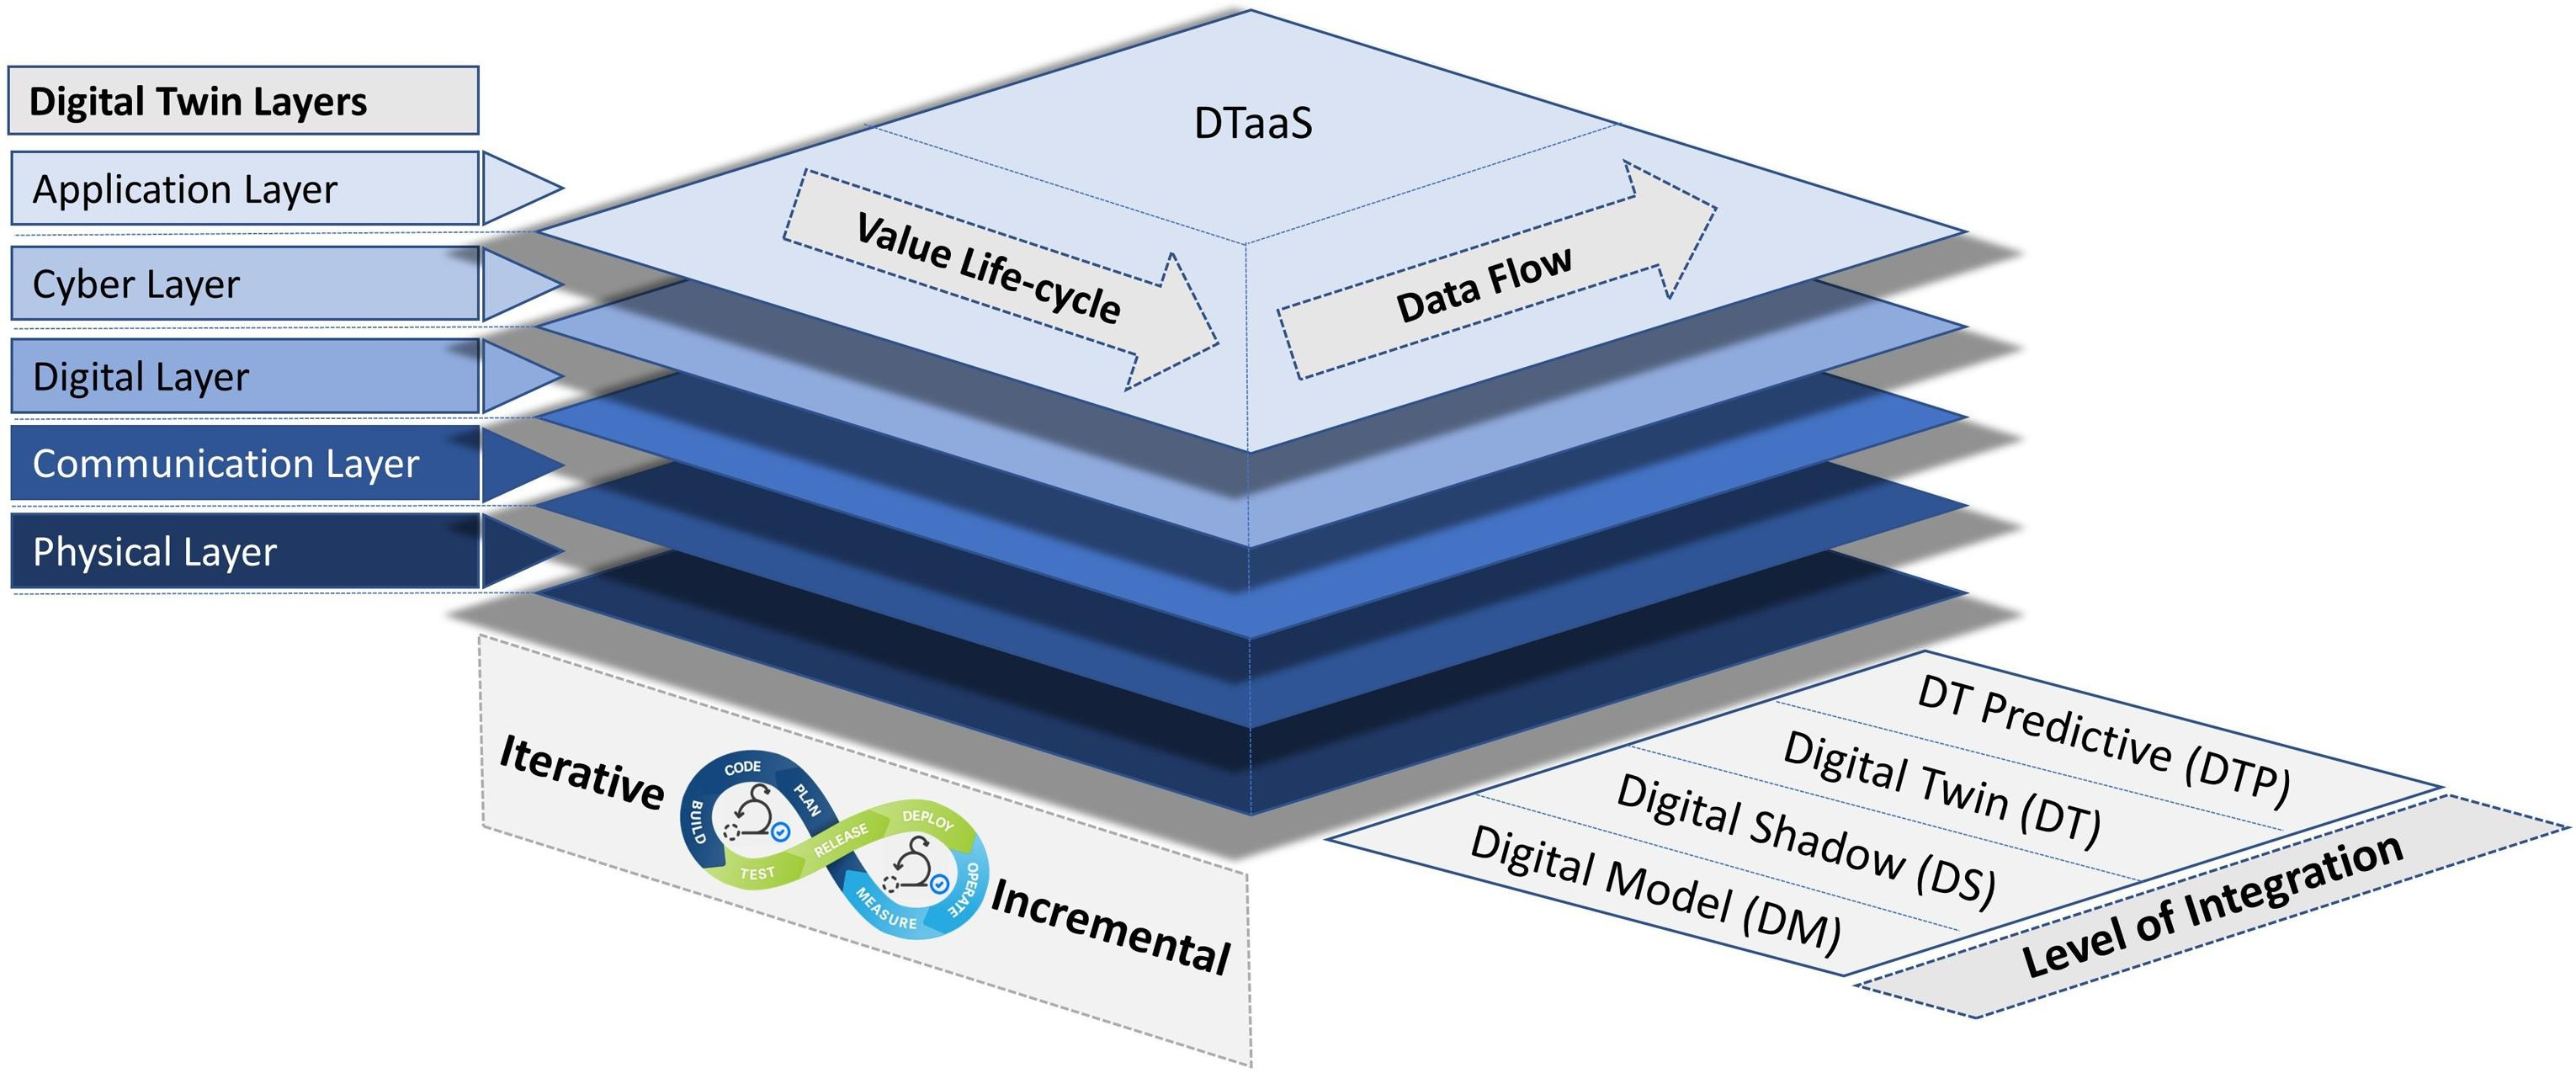
\includegraphics[width=\textwidth]{figures/dt-as-a-service.jpg}
    \caption{The DT-as-a-Service reference architecture, from \cite{aheleroff2021aei}.}
    \label{fig:dt-as-a-service}
\end{figure}

Layered and service-oriented architectures for \acp{DT} are the most popular in the literature.
%
These architectures support desired non-functional quality attributes such as performance efficiency, reliability and maintainability, but also compatibility with existing systems and scalability~\cite{ferko2022architecting}

On the functional side, \cite{dt-IoT-context-Minerva-2020} proposes a set of properties \ac{DT} should have, analyzing existing literature and implementations in the \ac{IoT} context.
%
The properties, summarized in \Cref{tab:minerva-properties} detail various aspects that characterize functional behavior of \acp{DT}.
%
Interestingly, such properties go beyond the generic definition of \ac{DT} as a virtual representation of a \ac{PA} and highlights the various capabilities that a \ac{DT} can provide to its users.

First, both the \ac{DT} and the \ac{PA} are required to be \emph{univocally identifiable} in order to establish a clear relationship between the two. This vision supports the possibility of having possibly multiple \acp{DT} representing the same \ac{PA} in different contexts or for different purposes.
%
Accordingly, the second important contribution is the emphasis on \emph{contextualization}. 
This shifts the focus from the ultra-realistic \ac{DT} envisioned by NASA to a more pragmatic approach where the \ac{DT} is representative of the \ac{PA} in a specific context,
hence possibly abstracting away details of the \ac{PA} that are not relevant for the intended use of the \ac{DT} in the target system.
%
Additional properties emphasize the dynamic nature of the \ac{DT} and its ability to reflect changes in the \ac{PA} (\emph{reflection}), in a timely manner (\emph{entanglement}), persisting over time (\emph{persistence}), memorizing past states (\emph{memorization}) and offering a reliable representation of the \ac{PA} (\emph{accountability}). 
%
Finally, the properties also highlight the ability of \acp{DT} to provide value to users through services (\emph{servitization}) such as aggregation of multiple assets (\emph{composability}), augmentation of the \ac{PA} capabilities (\emph{augmentation}), management of access control (\emph{ownership}), and anticipation of future states and behaviors of the \ac{PA} (\emph{predictability}).

\begin{table}[ht]
\centering
\caption{Characterizing Properties of \acp{DT}, defined in \cite{dt-IoT-context-Minerva-2020}.}
\renewcommand{\arraystretch}{1.3}
\begin{tabular}{p{3.5cm}|p{\dimexpr\textwidth-4.5cm\relax}}
\toprule
\midrule
\textbf{Property} & \textbf{Description} \\
\midrule
\toprule
{Contextualization} & A \ac{DT} models the \ac{PA} in a way that is representative with regard to the target context. \\
\hline
{Reflection} & A \ac{DT} reflects changes in the \ac{PA} in real-time. \\
\hline
{Replication} & A \ac{DT} replicates an object into different environments. \\
\hline
{Entanglement} & The degree to which a \ac{DT} is interconnected with its \ac{PA}. \\
\hline
{Persistency} & A \ac{DT} persists over time even when the \ac{PA} is not available. \\
\hline
{Memorization} & A \ac{DT} stores and allows retrieving past states and events. \\
\hline
{Composability} & A \ac{DT} can aggregate different assets or \acp{DT}. \\
\hline
{Accountability} & A \ac{DT} recovers from errors and maintains a reliable state.\\
\hline
{Augmentation} & A \ac{DT} can add new capabilities to the \ac{PA}.\\
\hline
{Ownership} & A \ac{DT} manages access control over its data and functionalities.\\
\hline
{Servitization} & A \ac{DT} provides services to its users.\\
\hline
{Predictability} & A \ac{DT} can anticipate future states and behaviors of the \ac{PA}.\\
\midrule
\bottomrule
\end{tabular}%
\label{tab:minerva-properties}
\end{table}



%=======================================================
\section{Enabling Technologies and Platforms}
%=======================================================

On a practical level, the implementation of \acp{DT} has been enabled by the convergence of various technologies.
%
This includes the proliferation of \ac{IoT} devices, 
advancements in Big Data analytics and \ac{AI}, 
and an increased availability of computing power to run simulations, 
which make possible to collect and analyze large amounts of data from the physical world, 
derive models of the \ac{PA} and execute them to obtain insights~\cite{qi2021enablingtechdt,Fuller_Fan_Day_Barlow_2020,Mihai_survey_enabling_2022}.

On the physical side, the availability of network-connected sensors and actuators enable the acquisition of real-time data from the \ac{PA}.
%
Sensing technologies for \ac{DT} broadly include classic \ac{IoT} techniques such as RFID, digital sensors,
but also computer vision and image processing.
%
In many cases, the data that can be automatically collected from the \ac{PA} is complemented by manual data entry, making the \ac{DT} interact with other information systems.
%
Sensing is followed by connectivity and data exchange, through a variety of communication protocols and network technologies.
%
\acp{DT} may need to operate with different data sources, each with its own communication protocol and data format.
%
Classic examples of \ac{IoT} communication protocols include MQTT, CoAP, HTTP, and WebSocket, but also industrial protocols such as OPC-UA and Modbus~\cite{Fortino_Savaglio_2023}. 
%
Finally, the physical layer includes a computing infrastructure that can span from the edge to the cloud, to support the data acquisition, processing and storage needs of the \ac{DT}.

On the virtual side, the \ac{DT} requires modeling techniques to represent its properties and behaviors.
%
Depending on the application domain this can range from geometrical and physical models, to behavioral models such as finite state machines or process models.
%
Models can be manually created by experts, or automatically derived from data through data-driven modeling and machine learning techniques~\cite{Tao_Xiao_Qi_Cheng_Ji_2022}.
%
Models can be used to simulate the behavior of the \ac{PA} with different simulation software.
%
The volume and variety of data that can be collected from the \ac{PA} and from the \ac{DT} models requires Big Data technologies to extract insights~\cite{Tao_Cheng_Qi_Zhang_Zhang_Sui_2018}. 
%
Finally, the \ac{DT} software needs to provide services to its users, including data visualization technologies, user interfaces and \acp{API} to interact with other software systems.
%
Some further include \ac{AR} and \ac{VR} technologies in the enabling technologies of \acp{DT} to provide immersive experiences to users and visualize \ac{DT}~\cite{Mihai_survey_enabling_2022}.

\todo{maybe a table or something to break the text... }

Due to the complexity of the technological stack required to implement \acp{DT}, the industry has seen the emergence of various supporting tools.
%
First examples of \ac{DT} development tools were developed by large industrial companies such as General Electric's Predix, Siemens MindSphere, PTC ThingWorx, and IBM Watson \ac{IoT}~\cite{Fuller_Fan_Day_Barlow_2020,Adamenko_Kunnen_Nagarajah_2020}.
%
Additionally, several simulation tools such as  ANSYS Twin Builder~\cite{ansys_twinbuilder}, SimuLink~\cite{mathworks_digitaltwin} and AnyLogic~\cite{anylogic_digitaltwin} started to include features to support \ac{DT} development. 
%
Many of these tools, emerging from industrial domains, are tailored to specific use cases and application domains.
%
Additionally, being proprietary software, they often lack openness and interoperability becoming closed silos from a broader system engineering perspective. 

More recently, cloud providers have started to offer so-called \emph{\ac{DT} platforms} such as Microsoft's \azureTwin{}\footnote{\url{https://azure.microsoft.com/en-us/services/digital-twin/}} and Amazon's \awsTwin{}\footnote{\url{https://aws.amazon.com/iot-twinmaker/}}.
%
These general-purpose platforms complement the existing cloud-based \ac{IoT} middlewares with specific features to support the implementation of \acp{DT}. 
This includes the ability to model assets with defined data schemas, providing identification and tracking state properties,
as well as tools to integrate data from various sources, and to grant access to the \ac{DT} data and functionalities through well-defined common \acp{API}.
%
Interestingly, these platforms put forth the idea of having multiple \acp{DT} connected together to represent a complex application domain. 
%
As an example, \azureTwin{} is based on the concept of a \emph{digital twin graph} where multiple \acp{DT} can be connected together to represent complex systems~\cite{Meijers_2022}.
%
Additionally, these platforms are not tied to specific application domains, paving the way for a broader adoption of the \ac{DT} concept. 

Last, but not least, open-source \ac{DT} platforms are emerging~\cite{Gil_Mikkelsen_Gomes_Larsen_2024}.
Among them, \ditto{}\footnote{\url{https://eclipse.dev/ditto/}} is a notable example, integrating with the Eclipse \ac{IoT} ecosystem. 
%
The platform allows storing and managing digital representations of \acp{PA}, providing a RESTful \ac{API} to interact with them. 
%
Other relevant examples from the academic community include
the \ac{DT}-as-a-Service platform proposed in \cite{Talasila_Gomes_Mikkelsen_Arboleda_Kamburjan_Larsen_2023} supporting developers in developing and sharing \acp{DT} by managing a combination of services including simulation models and data sources,
and TwinBase~\cite{Autiosalo_Siegel_Tammi_2021}, a platform to manage \ac{DT} models in the open Web with an implementation leveraging GitHub repositories to store and serve static \ac{DT} models.

The shift towards more general and open \ac{DT} platforms is reflecting the broader application of \acp{DT} beyond their original industrial context, as well as the need of integrating \acp{DT} in larger software ecosystems, instead of being closed in application silos. 

%=======================================================
\section{\aclp{DT} and \acl{AI}}
%=======================================================

As highlighted in the previous section, 
despite not being considered a core requirement when \acp{DT} were initially introduced,
\ac{AI} and machine learning techniques are increasingly being recognized as one of the fundamental enabling technologies for \acp{DT}~\cite{Kreuzer_Papapetrou_Zdravkovic_2024}.
%
This is due to the fact that the amount of data that can be collected from \acp{DT} is often too large and complex to be manually analyzed and interpreted. 
%
Hence, \ac{AI} techniques can be used to implement different \ac{DT} functionalities. 

In \cite{Minerva_Crespi_Farahbakhsh_Awan_2023}, the authors propose a classification of \ac{DT} based on the level of behavioral intelligence, correlating the different levels to different \ac{AI} techniques as shown in \Cref{fig:ai-dt-pentagon}.
%
They introduce four levels of \ac{DT} intelligence: 
\begin{itemize}
    \item \textbf{Passive} if the \ac{DT} purpose is only to provide a virtual representation of the \ac{PA} for monitoring and simulation purposes;
    \item \textbf{Predictive} if the \ac{DT} can forecast future \ac{PA} states and behaviors based on historical data and models;
    \item \textbf{Reactive} if the \ac{DT} can respond to changes in the \ac{PA} state by diagnosing issues and taking corrective actions using reasoning techniques;
    \item \textbf{Proactive or Autonomic} if the \ac{DT} can understand the \ac{PA} context and make decisions adapting to it to autonomously reach or maintain goals without human intervention.
\end{itemize}

\begin{figure}[ht]
    \centering
    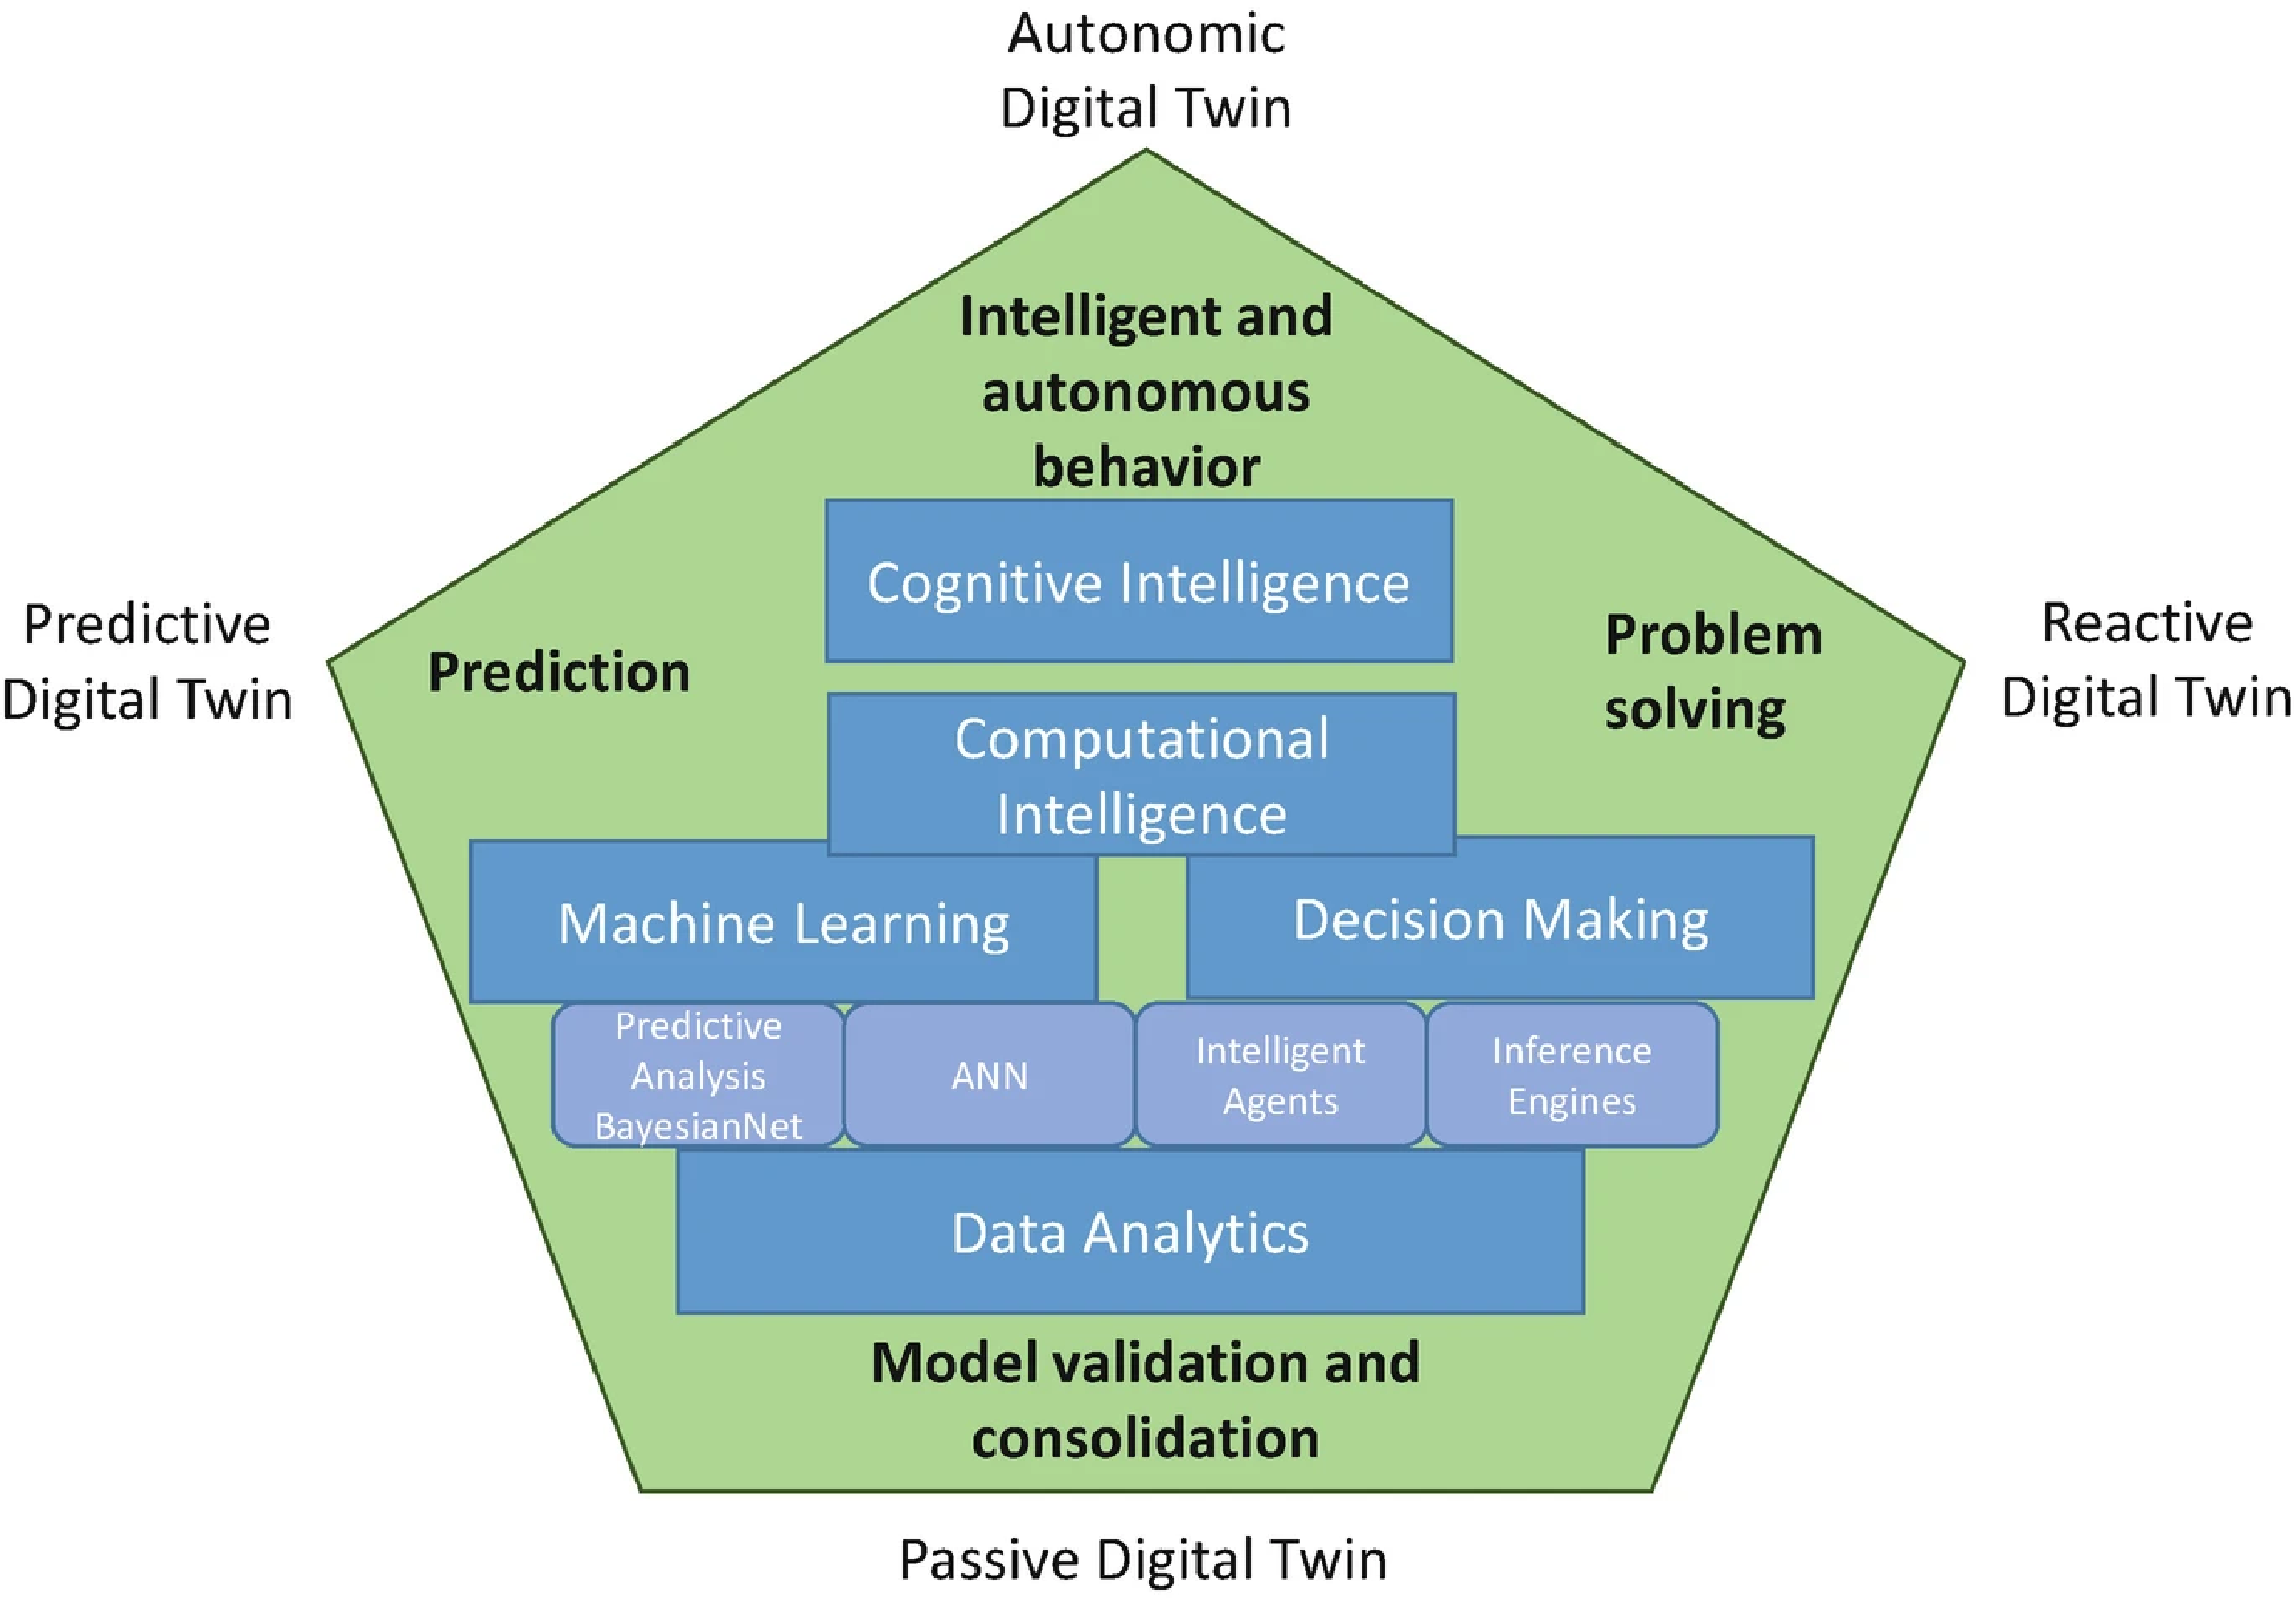
\includegraphics[width=0.9\textwidth]{figures/AI_DT_pentagon.pdf}
    \caption{Artificial intelligence with respect to \ac{DT} capabilities, from \cite{Minerva_Crespi_Farahbakhsh_Awan_2023}.}
    \label{fig:ai-dt-pentagon}
\end{figure}

Passive \acp{DT} can be supported by statistical data analytics techniques to create models of the \ac{PA}. 
%
Predictive \acp{DT} can leverage different techniques such as regression, time series analysis, deep learning but also fuzzy logic to implement the prediction capabilities. 
%
This of course requires the availability of historical data to train such models. 
%
Reactive \acp{DT} can instead use classification techniques, decision-trees and rule-based systems to implement decision-making. 
%
Finally, Autonomic \acp{DT} can combine different reasoning techniques with planning to implement self-adaptation and autonomous beavior.
%
This level of intelligence is often associated with the vision of \emph{Cognitive Digital Twins}~\cite{Zheng_Lu_Kiritsis_2022,Intizar_Ali_Patel_G_Breslin_Harik_Sheth_2021} in which the \ac{DT} has a strong degree of autonomy with respect to its \ac{PA} and can influence its behavior to achieve specific goals.
%
The technologies tied to this vision include knowledge representation, ontologies and reasoning, hence including the more symbolic side of \ac{AI} techniques, rather than only relying on data-driven techniques.



%=======================================================
\section{Digital Twin Interoperability}
%=======================================================

The rapid development of \ac{DT} technologies and the adoption of \acp{DT} in various domains has led to a fragmentation of the field. 
%
Moving on from the technological silos of the early \ac{DT} implementations towards a more service-oriented view of \acp{DT},
it is not surprising that interoperability is emerging as a key challenge for \acp{DT}~\cite{piroumian2021interoperability,Rebelo_Moreira_2024}. 


Interoperability is seen as a necessary condition for \ac{DT} maturity.
In \cite{Klar_Arvidsson_Angelakis_2024} the authors propose a general maturity assessment framework for \acp{DT}. 
\Cref{tab:dt-maturity} summarizes the proposed levels of maturity.


\begin{table}[htbp]
\centering
\renewcommand{\arraystretch}{1.2}
\begin{tabular}{c|p{2.8cm}|p{5cm}|p{4cm}}
\toprule
\midrule
\textbf{Level} & \textbf{State} & \textbf{Requirement} & \textbf{Enabled potential} \\
\midrule
\toprule
1 & Replication of assets & 
Digitization of physical assets and their state at moment of capture (e.g. 2D maps or 3D models) & 
Awareness of assets, rudimentary decision support \\
\hline
2 & Connection & 
Connect processes and models to static data and metadata of level 1 & 
Realistic simulations and asset planning \\
\hline
3 & Synchronization & 
Enrich with timely data (sensors and other IoT technologies) & 
Real-time situational awareness and immersive environments \\
\hline
4 & Interaction & 
Two-way data communication and interaction & 
Remote control of physical assets and processes \\
\hline
5 & Automation & 
Transparent explainable systems with broad control potential & 
Autonomous operations optimization and self-maintenance \\
\hline
6 & Interoperability & 
Highly linkable systems characterized by a high level of standardization, ontology definition, and semantic modelling & 
Joint decision-making among various systems, enhanced system of systems performance \\
\midrule
\bottomrule
\end{tabular}
\caption{Levels of \acl{DT} maturity from \cite{Klar_Arvidsson_Angelakis_2024}.}
\label{tab:dt-maturity}
\end{table}

Authors correlate level one and two to the Digital Model, level three to the Digital Shadow and level four and five to the Digital Twin concepts~\cite{kritzinger2018dtmanufacturing}.
%
Level six, which they identify as the highest level of maturity is tied to interoperability and envisions \emph{Connected Digital Twins} that can interact with each other to provide joint decision-making capabilities. 

In this context, interoperability is hence seen as a key enabler for the realization of \ac{DT}-based systems and integrate the \ac{DT} concept as a \ac{CPS} engineering paradigm. 
%
Accordingly, in \cite{Acharya_Khan_Päivärinta_2024}, the authors survey \ac{DT} literature to characterize interoperability in \ac{CPS} and \ac{DT} systems.
%
\Cref{fig:dt-interoperability-levels} visually summarizes the identified levels of interoperability in six levels: 

\begin{figure}[ht]
    \centering
    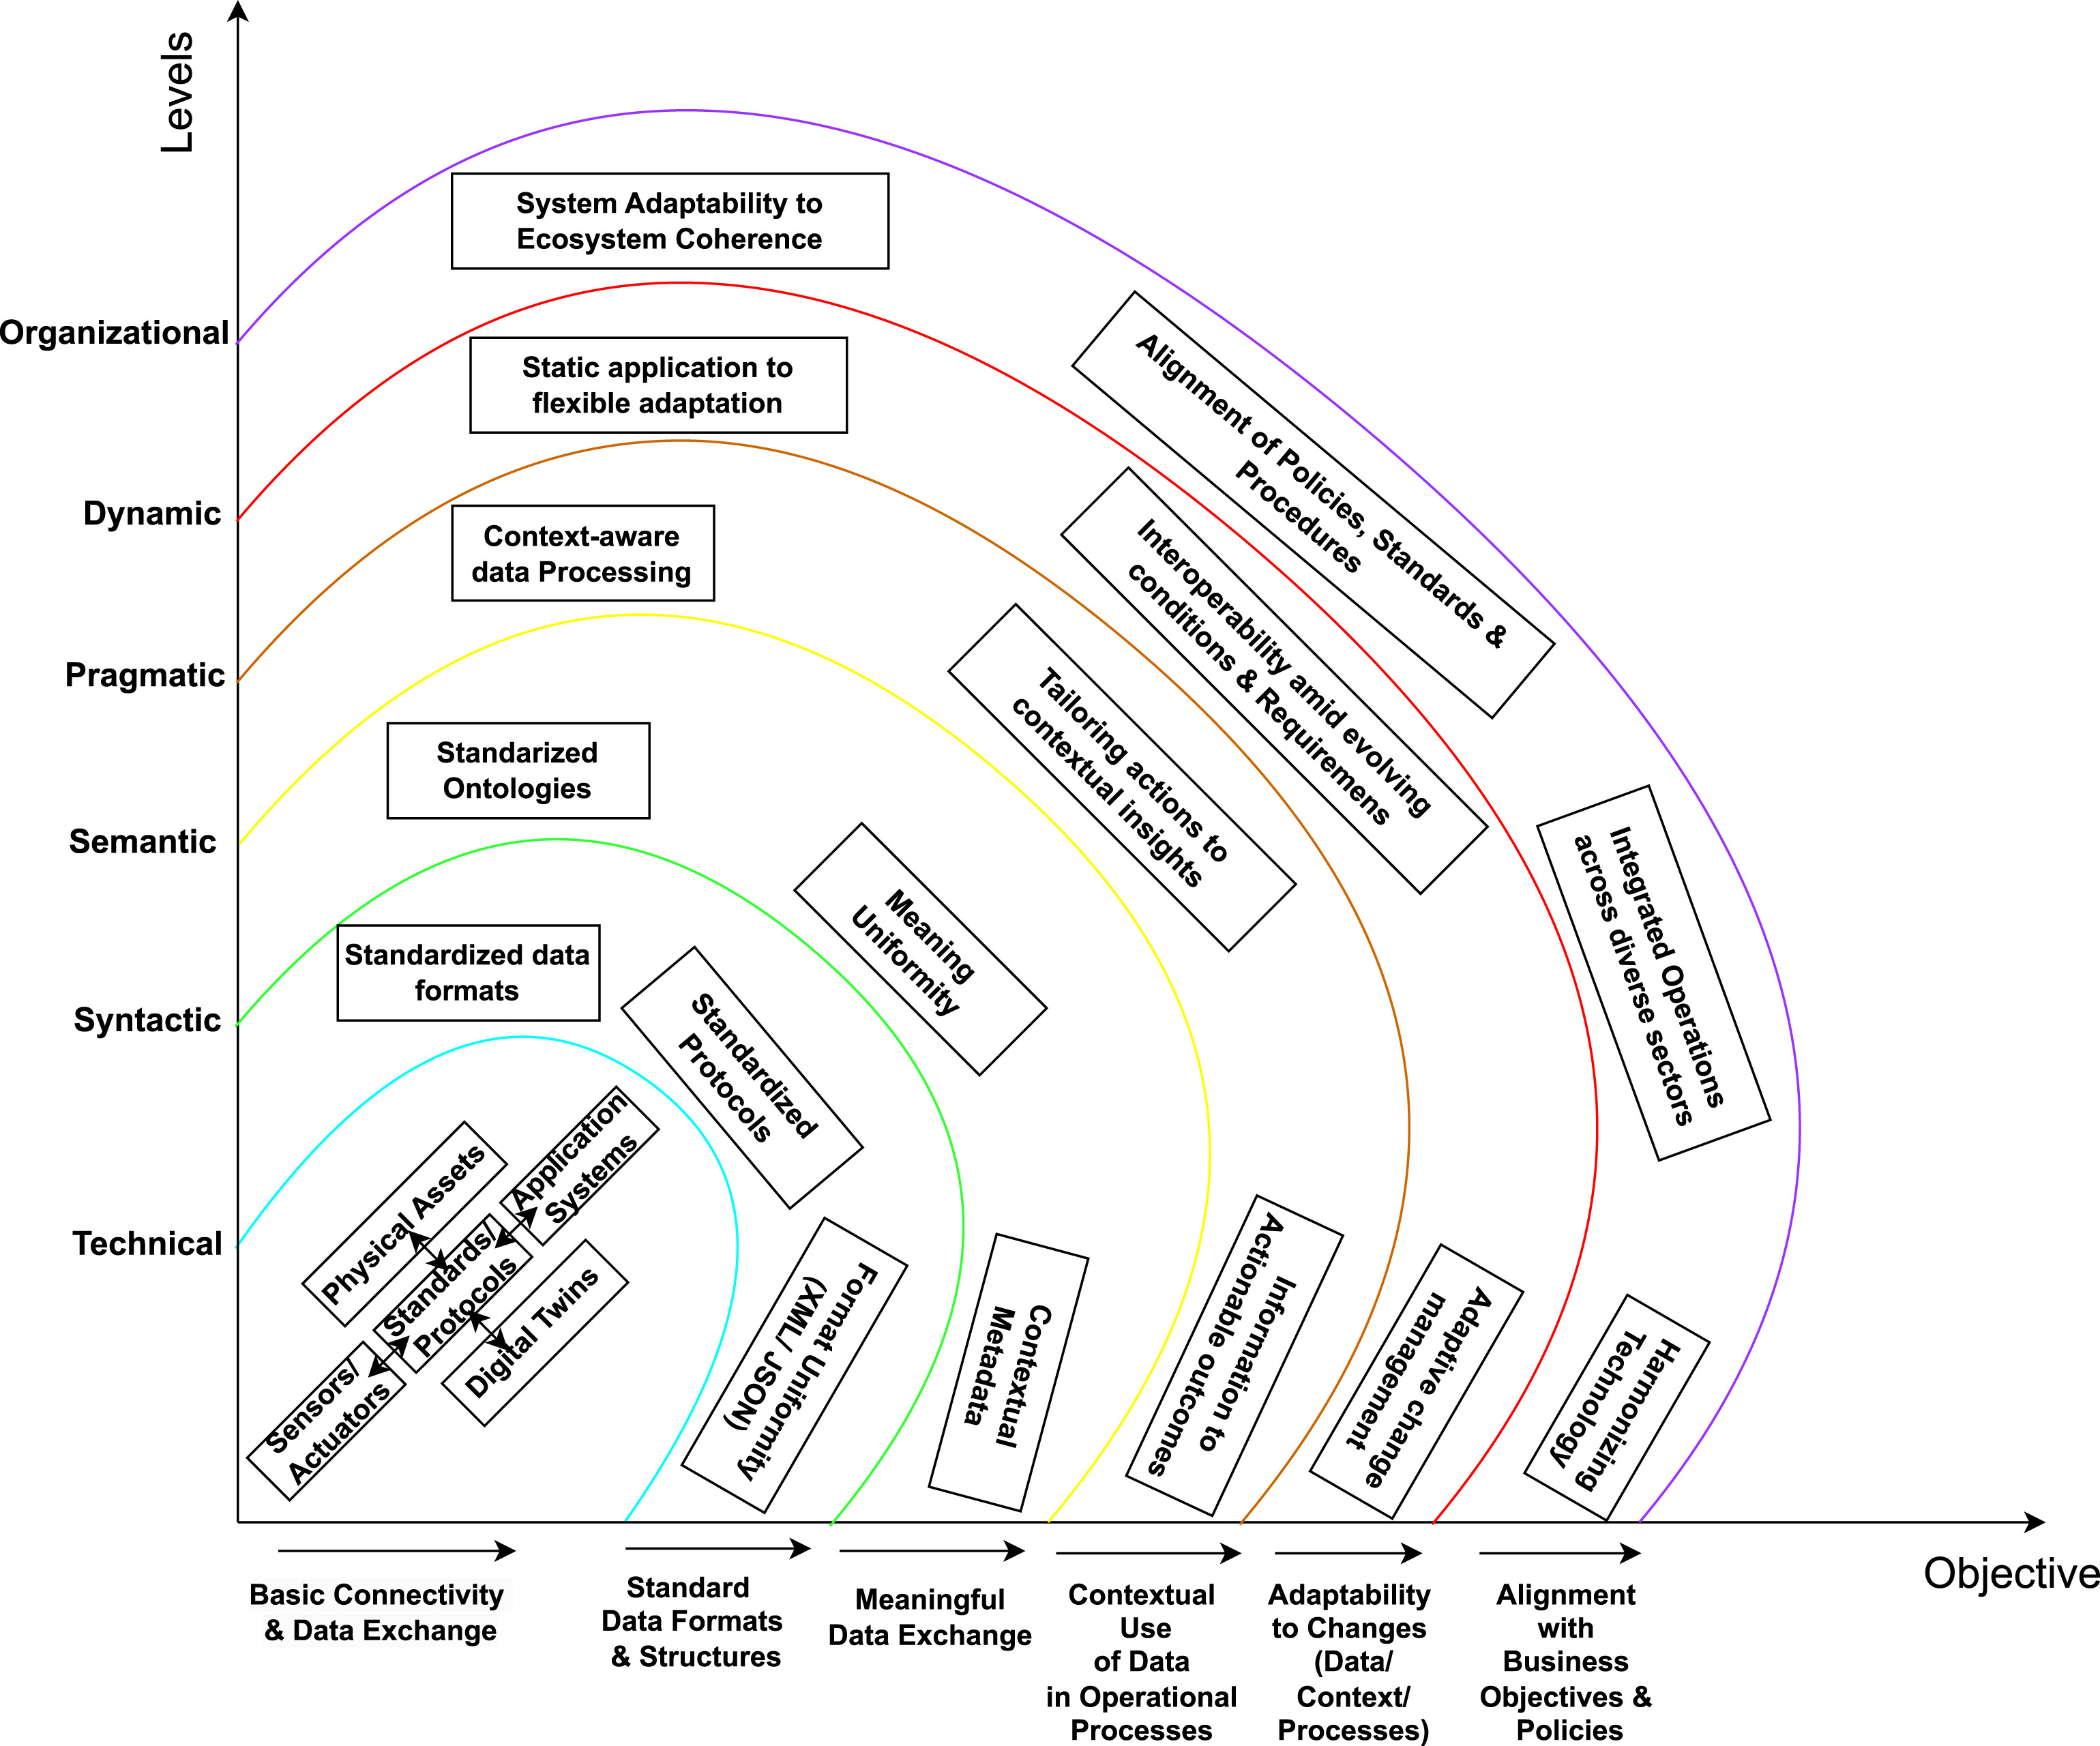
\includegraphics[width=\textwidth]{figures/interoperability-levels.jpg}
    \caption{Interoperability Levels in \acl{DT}, from \cite{Acharya_Khan_Päivärinta_2024}.}
    \label{fig:dt-interoperability-levels}
\end{figure}


\begin{enumerate}
    \item \textbf{Technical Interoperability} is the lowest level and refers to the ability of different systems to communicate and exchange data using common protocols and formats;
    \item \textbf{Syntactic Interoperability} refers to the ability of different systems to understand the structure and format of the exchanged data, enabling them to parse and interpret it correctly;
    \item \textbf{Semantic Interoperability} refers to the ability of different systems to understand the meaning of the exchanged data, enabling them to interpret it consistently;
    \item \textbf{Pragmatic Interoperability} refers to the ability of systems to understand context of the exchanged data and use it to 
    \item \textbf{Dynamic Interoperability} refers to the ability of different systems to adapt and evolve over time, enabling them to maintain interoperability in the face of changing requirements and technologies
    \item \textbf{Organizational Interoperability} refers to the ability of different organizations to work together effectively, through the adherence to standards and the integration of operations. 
\end{enumerate}
%

These studies highlight the importance of interoperability for the future of \acp{DT}, emphasizing the need for standardization and common frameworks to enable seamless integration of \acp{DT} in larger systems. 
%
The envisioned ultimate goal, tends towards \acp{DT} as building-blocks of more complex systems, interacting with each other to provide additional value. 

Of course, there are significant challenges to achieve this vision.
%
In \cite{Klar_Arvidsson_Angelakis_2024}, the authors identify the lack of trust as a key barrier to interoperability, especially for an organizational level as the exchange of data is often perceived as a loss of competitive advantage.
%
Initiatives such as the European data space~\cite{Braud_Fromentoux_Radier_Le_Grand_2021} are trying to address this issue by proposing a federated data infrastructure where data can be shared in a secure and controlled manner.

Other than societal challenges, technical issues such as data silos, proprietary formats, and lack of common standards further complicate interoperability efforts.
%
Standardization initiatives such as the one from \ac{ETSI}~\cite{etsi_TR_103844_v1.1.1_2023} aim to address these challenges by providing guidelines and frameworks for interoperable \acp{DT}.
%
Different challenges arise at different levels of interoperability~\cite{Klar_Arvidsson_Angelakis_2024}.

At the technical level, a plethora of standards originally developed within the industrial \ac{IoT} domain are being proposed to address the communication and data exchange needs of \acp{DT}~\cite{Barnard_2024}.
%
Examples are the \ac{AAS}~\cite{platform_i40_aas_part1_v2}, the \ac{OPC-UA}~\cite{mahnke2009opc}, and \ac{AML}~\cite{DBLP:conf/etfa/DrathLPH08}.
%
These standards, given their different origins and motivations, cover different aspects of a \ac{DT}~\cite{Barnard_2024} and are generally tailored to a specific problem, namely \ac{AAS} focuses on creating a representation of an asset through its static and dynamic properties, operations and services;
\ac{OPC-UA} primarily serves as a secure and efficient \ac{M2M} communication protocol and data model; and \ac{AML} captures the geometry, topology, and behavior of machines in automation processes.


At the semantic level, authors recognize the role of shared semantic models to provide common understanding of the exchanged data.
%
In this setting, ontologies and \acp{KG} are seen as essential tools to implement \acp{DT}~\cite{Karabulut_Pileggi_Groth_Degeler_2024}. They can provide a common vocabulary and shared understanding of an application domain, fostering interoperability, explainability and reasoning capabilities.
%
The survey finds that most \ac{DT} implementations use ontologies to represent the physical layer as it is the one more tied to the application domain. Few leverage ontologies to exchange data and build \acp{KG} to share the \ac{DT} knowledge, limiting their interoperability potential~\cite{Karabulut_Pileggi_Groth_Degeler_2024}.

%
% A different approach to \ac{IoT} interoperability is the aforementioned W3C \ac{WoT} which provides a general purpose model to integrate multiple \ac{IoT} devices, using Web principles to support the discovery of capabilities described through \acp{TD}.
% %
% Differently from the other approaches, the \ac{WoT} focuses on modeling interactions with devices, allowing to translate \acp{API} from machine-specific to Web-based protocols.

% Given the different nature of these standards, they can be viewed as complementary rather than competing against each other.
% %
% There have been integration efforts in order to leverage their different strengths. For instance, \ac{OPC-UA} has been integrated with web technologies~\cite{DBLP:journals/csi/CavalieriSS19} to support direct integration with web clients, operations in \ac{AAS}~\cite{platform_i40_aas_part1_v2} and affordances in \ac{WoT}\footnote{\url{https://profiles.opcfoundation.org/workinggroup/97}} can have an \ac{OPC-UA} protocol bindings, and \ac{AML} specifications can be linked to \ac{AAS} to have a coherent view of the involved assets~\cite{DBLP:conf/etfa/DrathRH19,DBLP:conf/indin/WengerZ018}.
% %
% In this view, the Semantic Web technologies adopted in the \ac{HWoDT} approach can be integrated on top of existing standards and complement their features.

% The Semantic Web excels at general-purpose knowledge representation, and integration of such heterogeneous knowledge under a uniform interface.
% %
% Additionally, it enable reasoning through ontological inference and expressive queries across concepts, supporting use cases that have limited support when using the aforementioned standards alone (see \cref{tab:interop_comparison}, Querying and Data access).
% %
% It is then not surprising that alignment between Semantic Web technologies and industrial standards are being investigated, highlighting similarities between e.g., \ac{OPC-UA}~\cite{DBLP:conf/etfa/MajumderWD19,DBLP:conf/etfa/PerzyloP0K19} and \ac{AAS}~\cite{DBLP:conf/icphys/BedenCB21, platform_i40_aas_part1_v2} data models, to benefit from these features.

%=======================================================
\section{Towards \aclp{DTE}}
%=======================================================

As discussed in the previous sections, \acp{DT} are evolving from the original view of virtual copies of physical products, to serve as a general-purpose engineering abstraction for the strategic design and development of \acp{CPS}.
%
This shift is reflected by both technological advancements with the emergence of \ac{DT} platforms that support the management of multiple \acp{DT}, and the increasing attention to interoperability to enable \acp{DT} to be integrated in larger systems.


Complex \acp{CPS}, in fact, typically consist of interrelated assets whose connections can change dynamically.
%
These relationships are currently difficult to track and model with a single \ac{DT}, hence several approaches are proposing to consider a more collective dimension in which each asset is modeled with its own \ac{DT}, and the overall system is modeled as an \emph{ecosystem} of interconnected \acp{DT}~\cite{web-of-dt-ricci-2022}.
%
\emph{\ac{DTE}}, which are the core concept explored in this thesis, are hence emerging as a key abstraction to address the challenge of effectively model complex \acp{CPS} through a set of interconnected \acp{DT}.
%
The call to \emph{``make more \aclp{DT}''}~\cite{nature_make_moredt} is hence opening a perspective in which \acp{DT} are pervasively used to model strategic \acp{PA} and their interaction becomes crucial to effectively leverage their potential in complex scenarios.

The idea of \ac{DTE} can be traced back to the concept of \emph{Digital Twin Aggregate} introduced by Grieves~\cite{Grieves_2023} which understood the potential of aggregating multiple \acp{DT} instances.
%
In that vision, though, the aggregate was composed of multiple \acp{DT} of the same type of asset, to observe the behavior of different instances of the same product and capture collective trends.

The more modern interpretation of \ac{DTE} can be derived, instead, from the United Kingdom's \textit{National Digital Twin} program~\cite{bulter2018geminiprinciples}.
%
As described in \cite{kendall2021ndt} the National Digital Twin is \emph{``an ecosystem
of digital twins and the protocols by which
they can be integrated securely and
resiliently''}.
%
Finalized at the tracking of the national built environment, the initiative fostered the development of a \ac{DT} integration framework to share and exchange data across different stakeholders.
%
Although the program was focused on a specific domain, the underlying idea of composing an ecosystem of interconnected \acp{DT} rather than a monolithic put forth by the \emph{Gemini principles}~\cite{bulter2018geminiprinciples} can be generalized to other applications.
%
Today, \ac{DTE} are hence envisioned as systems where multiple \emph{different} \acp{DT} are interconnected to model complex scenarios spanning different domains and organizations.


% Building on this idea, recent research proposals advocate modeling such complex scenarios as \textit{\dteco{}}~\cite{web_of_dt}, which consist of a dynamic set of \acp{DT}, each individually mirroring a specific \ac{PA}.
% %
% Hence, \acp{DT} become building blocks to model portions of the real world, including every facet, ranging from people to objects and processes.




% %s
% The \textit{\acf{WoDT}}~\cite{web_of_dt} idea, built on this rationale, envisions ecosystems of connected \acp{DT} where each strategic \ac{PA} is modeled with at least one corresponding \ac{DT} which reflects, augments, and exposes its state, services, and \textit{relationships}.
% %
% The resulting \dteco{s} capture the interconnected nature of the physical world, creating an open, distributed, and dynamic service-oriented layer that models entire portions of the real world (\Cref{fig:wodt}).
% %
% Applications, especially smart applications and multiagent systems, can leverage this \ac{DT} layer to access, navigate, reason, and act upon the physical world~\cite{web_of_dt}.
% \begin{figure}[ht]
%   \centering
%   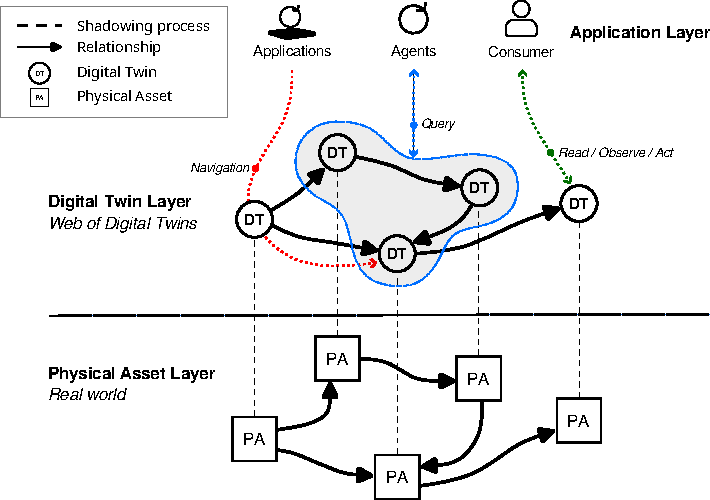
\includegraphics[width=0.9\linewidth]{figures/wodt.pdf}
%   \caption{A \dteco{} in the \ac{WoDT} vision. It depicts the typical \ac{WoDT} layered structure. The \textit{Physical Asset Layer} is mirrored with a \dteco{} in the \textit{Digital Twin Layer}, whose services are leveraged by the \textit{Application Layer}.}
%   \label{fig:wodt}
% \end{figure}
% The resulting holistic conceptualization enables services that extend beyond the boundaries of a single \ac{DT} to encompass the ecosystem as a whole, improving the design of large-scale systems.
% %
% Modeling cross-domain and cross-organization scenarios with an open-system perspective, a general-purpose metamodel is required.
% Hence, a \ac{DT} in the \ac{WoDT} is defined through the following metamodel composed of:
% \begin{inlinelist}
%     \item \textit{Properties} that represent the observable attributes of the \ac{PA},
%     \item \textit{Relationships}: that reflect, at the \ac{DT} level, the connections between the \acp{PA} as links to other \acp{DT},
%     \item \textit{Actions}: that can be invoked to modify the state or behavior of the \ac{PA}, and
%     \item \textit{Events}: exposing notifications about the \ac{PA}.
% \end{inlinelist}

% Reflections in the context of a single \ac{DT} must be extended and enriched, considering the distributed nature of \dteco{s}~\cite{web_of_dt}.
% %
% Heterogeneity is crucial when considering a pervasive softwarization of the physical world across different domains and organizations \cite{tao2019makemoredt, bulter2018geminiprinciples}.
% Recently, approaches to design \dteco{s} in heterogeneous settings have been proposed~\cite{giulianelli2024models}.
% %
% However, to support the entire journey that leads developers to the deployment of \dteco{s}, a wider spectrum of challenges must be considered.
% %
% The overall picture encompasses the potential to have distributed \dteco{s} where \acp{DT} are developed with heterogeneous technologies deployed across different network layers, ranging from the edge to the cloud, to achieve the desired application goals.
% %
% This fragmentation hinders infrastructure management and \ac{DT} consumption, slowing down the application layer.
% %
% For \acp{DT} and \dteco{s} to be successfully exploited as an effective cyber-physical abstraction layer, the deployment complexities must be adequately supported, allowing application designers to focus on core functionalities.



% While the value of individual \acp{DT} is recognized as strategic for improving decision-making, \ac{CPS} often involve interconnected assets whose interactions may emerge only from a holistic view~\cite{JIA2022101706,JIA2023101915}.
% %
% The cardinal role of the \emph{service} dimension naturally leads to leveraging multiple \acp{DT} to model complex scenarios. 
% This aligns with the \emph{DT-as-a-service} view~\cite{aheleroff2021aei,talasila2025simulation} which fosters the composition of \acp{DT} and services in complex software ecosystems~\cite{human2023dtsoa}.

% Recent proposals target the development of \dteco{s}, where multiple \acp{DT}
% -- each representing individual \acp{PA} --
% support together applications and services that would simply not be achievable considering only isolated DTs~\cite{council2022geminipaperswhat,council2022geminipaperswhy}.
% %
% Among those, we highlight the efforts of the Digital Twin Consortium\footnote{\url{https://www.digitaltwinconsortium.org/}}
% and the United Kingdom's \ac{NDT} programme~\cite{kendall2021ndt}
% who were among the first dedicated activities advocating for the development of standards for \dteco{s} to achieve \ac{DT} interoperability.
% %
% Regardless of these and other ongoing efforts (e.g. \cite{iso2023concepts}, \cite{etsi2023tr103844}), interoperability is still considered one of the main challenges for achieving mature \dteco{s}~\cite{Klar_Arvidsson_Angelakis_2024,Acharya_Khan_Päivärinta_2024}

% Addressing this challenge, the \emph{\acf{WoDT}}~\cite{ricci2022wodt} puts forth a conceptual proposal for an open, distributed, and dynamic ecosystem of connected \acp{DT} adhering to a general-purpose metamodel composed by: 
% \begin{inlinelist}
%     \item \emph{properties} which are observable attributes of the \ac{PA};
%     \item \emph{relationship} representing connections between \acp{PA} as links to other \acp{DT};
%     \item \emph{actions} representing operations which can be invoked to modify the state or behaviour of the \ac{PA};
%     \item \emph{events} to capture notifications about the \ac{PA}
% \end{inlinelist}
% Still, the practical challenge of composing heterogeneous \emph{existing} \acp{DT} based on this meta-model is not addressed.
% Our proposal fills this gap by leveraging hypermedia-based interoperability to apply the \ac{WoDT} conceptual model to heterogeneous \dteco{s}.


\note{From platforms to ecosystems}

\note{National Digital Twin}

\note{Web of Digital Twins}


\begin{figure}[ht]
    \centering
    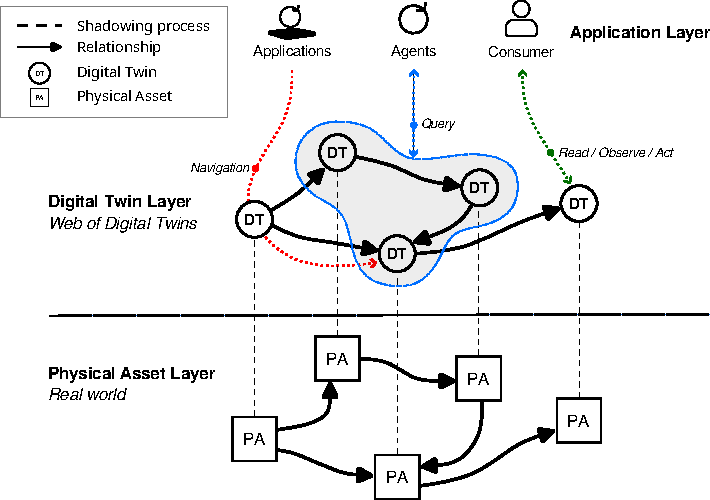
\includegraphics[width=\textwidth]{figures/wodt.pdf}
    \caption{Conceptual model of the \acl{WoDT}.}
    \label{fig:dt-wodt-model}
\end{figure}


%=======================================================
\section{Final Remarks}
%=======================================================

This chapter provides an overview of the research landscape around \acp{DT}.
 